\documentclass[tikz]{standalone}
\usetikzlibrary{arrows,angles,quotes,calc,decorations.pathreplacing}
\begin{document}
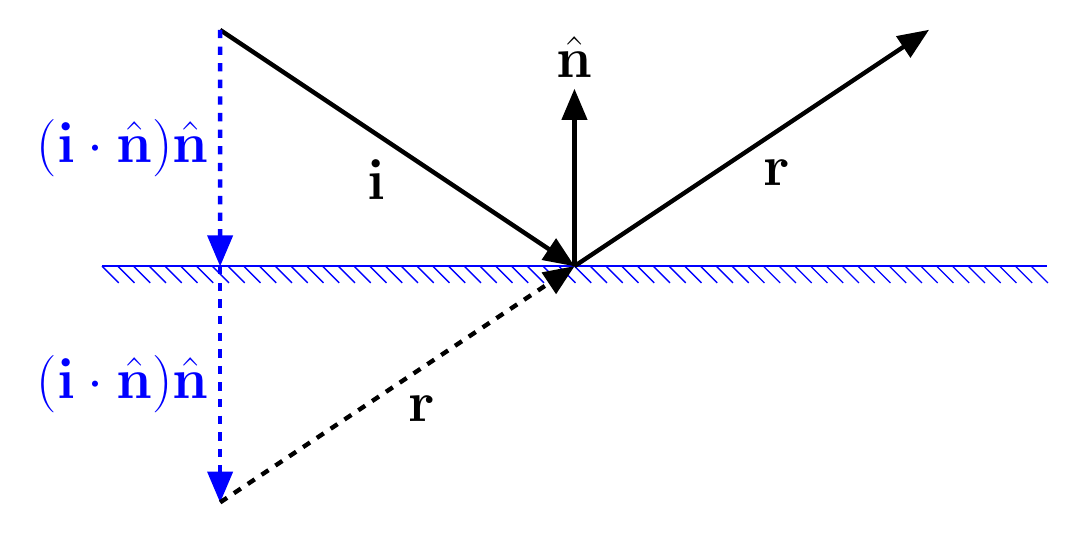
\begin{tikzpicture}[>=triangle 45,line width=1.6pt,scale=1.5,font=\fontsize{20pt}{0},
    interface/.style={
        postaction={draw,decorate,decoration={border,angle=-45,
                    amplitude=0.3cm,segment length=2mm}}}]
  \coordinate (O) at (0,0);
  \coordinate (V) at (-3,2);
  \coordinate (R) at (3,2);
  \coordinate (N)  at (0, 1.5);
  \draw[blue,line width=.5pt,interface](-4,0)--(4,0);
  \draw[->] (O) -- (N) node[anchor=south] {$\hat{\mathbf{n}}$};
  \draw[->] (V) -- (O) node[midway, anchor=north east] {$\mathbf{i}$};
  \draw[->] (O) -- (R) node[midway, anchor=north west] {$\mathbf{r}$};
  \draw[->, blue, style=dashed] (V) -- (-3, 0) node[midway, anchor=east] {$(\mathbf{i} \cdot \hat{\mathbf{n}})\hat{\mathbf{n}}$};
  \draw[->, blue, style=dashed] (-3, 0) -- (-3, -2) node[midway, anchor=east] {$(\mathbf{i} \cdot \hat{\mathbf{n}})\hat{\mathbf{n}}$};
  \draw[->, style=dashed] (-3, -2) -- (O) node[midway, anchor=north west] {$\mathbf{r}$};
\end{tikzpicture}
\end{document}
